\documentclass{article}
\usepackage[utf8]{inputenc}
\usepackage{graphicx}
\usepackage{fancyhdr}
\usepackage{verbatim}
\pagestyle{fancyplain}
\author{Mikkel, Jannik, Rune \& Rasmus}
\date{\today}
\lhead{Mikkel, Jannik, Rune \& Rasmus}
\rhead{\today}
\begin{document}

\section{Eksperimentdesign}

\subsection{Tidsmåling}

\subsection{Realisme}


\subsection{Andre Parametre}

\subsection{Tese}

\section{Implementation}

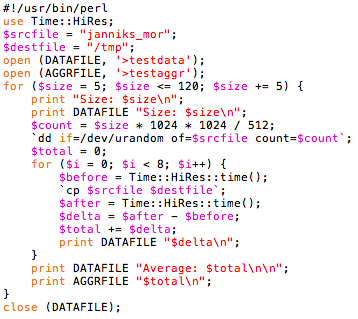
\includegraphics[width=4in]{kode.png}

\subsection{Omstændigheder}

\subsection{Graf}

\begin{figure}
	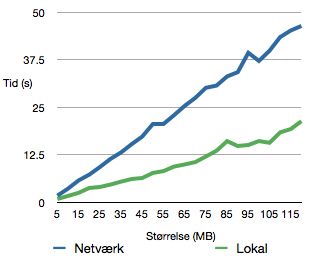
\includegraphics[width=4in]{ploto.png}
	\caption{Hej}
	\label{ploto}
\end{figure}

\begin{figure}
	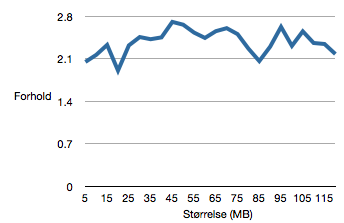
\includegraphics[width=4in]{plotforhold.png}
	\caption{Hej}
	\label{plotforhold}
\end{figure}

\subsection{Teseoverlevelse}

\subsubsection{i}

\subsubsection{ii}

\section{Ræssonnering}

\subsection{a}
\subsection{b}
\subsection{c}

\section{4...}

\begin{comment}

\begin{frame}{Tese}
Båndbredden over netværk er langt højere end båndbredden til en harddisk så hvis man skriver tilstrækkeligt store filer til en disk vil der ikke være forskel på skrivehastigheden mellem en netværksforbundet og en lokal harddisk.\\
$$ $$
Bemærk: Der vil blive målt skrivninger og ikke læsninger.
\end{frame}


\begin{frame}{Planlægning}
\begin{itemize}
\item Eksperimentet
\begin{itemize}
\item Overføre filer af forskellige størrelser lokalt og over netværk.
\item Filer af størrelser fra 5 MB til 120 MB med 5 MB intervaller.
\item Filerne består af tilfældigt indhold af de angivne størrelser.
\item Netværkskabel over trådløst netværk.
\item Lille netværksserver med harddisk på et hjemmenetværk.
\end{itemize}
\item Fejlkilder
\begin{itemize}
\item Caching
\item CPU som flaskehals
\item Hardware
\item Netværksbelastning
\item Andre processer / forstyrrelser
\item Software til montering af filsystem
\item Netværksudstyr (firewall / router)
\item Afstand
\end{itemize}
\end{itemize}
\end{frame}


\begin{frame}{Implementering}
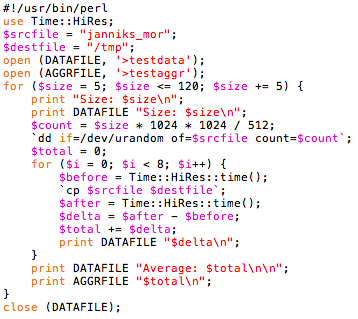
\includegraphics[width=3in]{kode.png}
\end{frame}


\begin{frame}{Resultater}
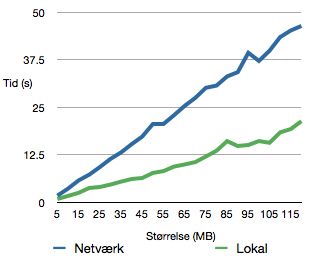
\includegraphics[width=3in]{ploto.png}
\end{frame}

\begin{frame}{Forhold}
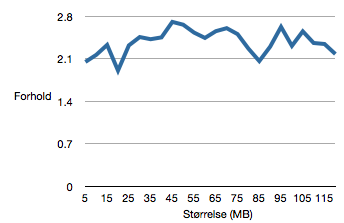
\includegraphics[width=3in]{plotforhold.png}
\end{frame}

\begin{frame}{Konklusion \& Perspektivering}
\begin{itemize}
\item \textit{ Alt andet lige holder tesen ikke.}
\item Overførslen til en lokal harddisk er op til dobbelt så hurtig som til en harddisk på et lokalt netværk.
\item Det er muligt at det vil se anderledes ud med større filer, men ingen tendens.
\item Ændre rækkefølge på tests så der alterneres mellem størrelser på de overførte filer frem for at der uploades hver størrelse 10 gange efter hinanden.
\item Hvorfor skulle det hjælpe med større filer?
\end{itemize}
\end{frame}

\end{comment}

\end{document}
